\chapter{Methods}
\label{chapter4}
A typical approach of using planning for exploration would consist of sampling plans, following them, realising their correctness through experience, and updating the model accordingly. However, since we know that all models are inaccurate, it's very possible that the optimal policy may never be discovered in this way. In order to mitigate these inaccuracies, and enable the optimal policy to be discovered, we suggest various frameworks that enable the planner to hypothesise, through reasoning, changes to the model that would be beneficial; that would lead to a better policy than the current one. The correctness of these changes is then realised through experience. To enable the planner to hypothesise these changes, we equip it with additional actions which we denote \textbf{Meta Actions}, which when called upon do not cause the agent to act in the environment but rather affect the model. This is an optimistic approach, but not over-optimistic where the agent will hallucinate, since the changes are driven by reasoning. The concept of "optimism in the face of uncertainty" is present, except we are almost always in a state of uncertainty due to the inevitable inaccuracies of the model. Given sufficient planning steps, with this method the agent would explore all states that could possibly be on the optimal path, inducing an envelope that is explored between the start and goal state.

\begin{figure}[h!]
    \centering
    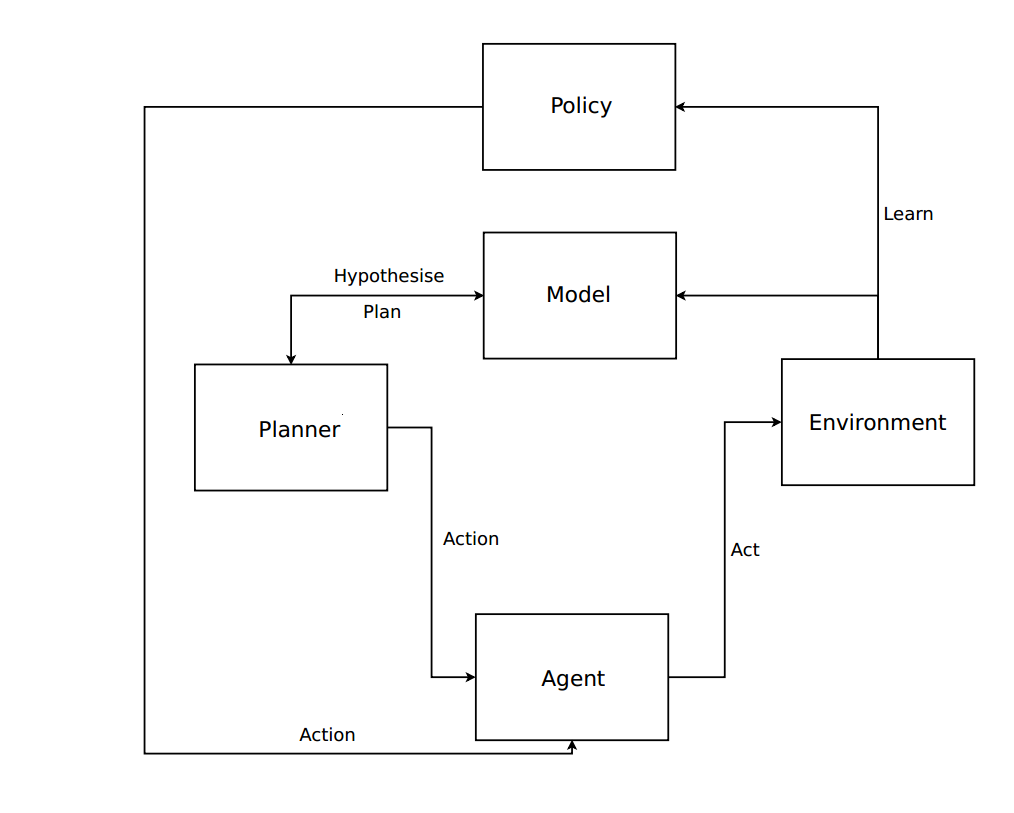
\includegraphics[max size={\textwidth}{\textheight}]{report/assets/diagram.png}
    \caption{Framework}
    \label{fig:framework}
\end{figure}

\begin{figure}[h!]
    \centering
    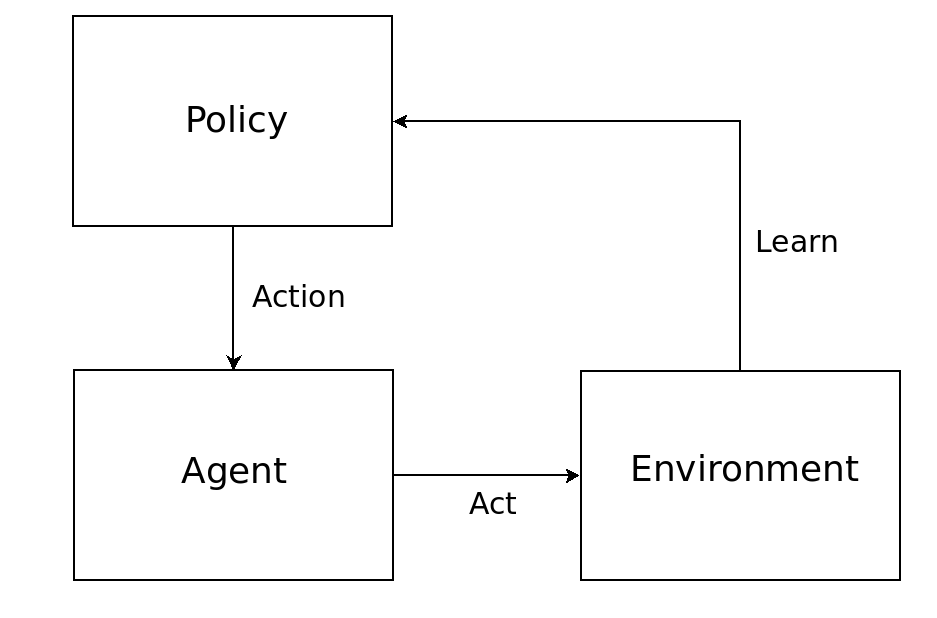
\includegraphics[max size={\textwidth}{\textheight}]{report/assets/rl_diagram.png}
    \caption{Framework}
    \label{fig:framework}
\end{figure}

% The core of this work is to follow a model-based RL approach, computing plans from a (inherently inaccurate) model to guide guide exploration, updating the model where necessary. What differentiates this from other works, highlighted in Chapter 2, is the additional actions exposed to the planner, that don't actually affect the environment, but rather the model; we deem these \textbf{Meta Actions}. The main idea is that the Planner can use these Meta Actions to hypothesise changes to the model that would be of most benefit, in this sense the approach is optimistic. The hypotheses are driven by reasoning.
\section{Meta Actions}
A Meta Action is an action which does not affect the environment in any way, thus the agent receives no observation or reward upon taking it, but rather it affects the model directly. For the Planner to suggest a Meta Action, it must be admissible, feasible and reasonable.
\subsection{Admissable}
A Meta Action is \textbf{admissable} if applying it to the model leads to what seems like a better plan. If applying the Meta Action does not result in any benefit to the planner, but rather it negatively affects the planner, then it should not be called.
\subsection{Feasible}
A Meta Action is \textbf{feasible} in the deterministic case if 1) the corresponding state or transition has not been previously observed 2) the Meta Action has not been previously called on the corresponding state or transition. For the stochastic case, a Meta Action is feasible if just 2 holds.
\subsection{Reasonable}
Since the change to the model that would most benefit the Planner is always to add a transition from the current state to the goal state, we need to add a constraint to what Meta Actions can be called, otherwise this results in random-walk-like behaviour.
For instance, Meta Actions can be learned; when we realise differences between the environment and the model, we can learn this difference as a Meta Action. Otherwise, reasonability can be something that is embedded directly in the model. Thus, a Meta Action is \textbf{reasonable} if it has been directly learned through experience or it is embedded in the model by-hand.
\section{Frameworks}
The high-level idea described above led to various frameworks being developed. The underlying concept of allowing the planner to hypothesise changes to the model is present throughout all of the frameworks, but the ways in which the planner decides which change is most beneficial differs, and in some places simplifications are offered for differing domains (deterministic vs stochastic). Each framework will be presented and highlighted here.
\section{A High Level Example}
\subsection{RL-A* (Deterministic)}
A simple model-based RL implementation; the agent explores by planning on the model, and learns the model as it does so.
\subsection{RL-A* Meta (Deterministic)}
A simple model-based RL implementation; the agent explores by planning on the model, and learns the model as it does so.
Additionally, the planner is equipped with the following actions: RemoveObstacle, AddObstacle, DecreaseReward, IncreaseReward.
\subsection{RL-A* Meta, with short-term memory (Stochastic)}
A simple model-based RL implementation; the agent explores by planning on the model, and learns the model as it does so.
Additionally, the planner is equipped with the following actions: RemoveObstacle, AddObstacle, DecreaseReward, IncreaseReward. The planner approximates a deterministic model which it plans on. To allow for sufficient exploration, the agent has a short-term memory, encouraging it to try Meta Actions again, where it wouldn't be able to do so in the deterministic case.
\subsection{RL-VI (Deterministic)}
A model-based RL implementation; the agent explores by planning on the model, and learns the model as it does so.
\subsection{RL-VI Meta (Deterministic)}
A model-based RL implementation; the agent explores by planning on the model, and learns the model as it does so.
Additionally, the planner is equipped with the following actions: AddTransition, RemoveTransition, DecreaseReward, IncreaseReward.
\subsection{RL-VI (Stochastic)}
A model-based RL implementation; the agent explores by planning on the model, and learns the model as it does so.
\subsection{RL-VI Meta (Stochastic)}
A model-based RL implementation; the agent explores by planning on the model, and learns the model as it does so.
Additionally, the planner is equipped with the following actions: IncreaseTransitionProbability, DecreaseTransitionProbability, DecreaseReward, IncreaseReward.
\subsection{RL-VI Meta, with learning Meta Actions (Stochastic)}
A model-based RL implementation; the agent explores by planning on the model, and learns the model as it does so.
Additionally, the planner is equipped with the following actions: IncreaseTransitionProbability, DecreaseTransitionProbability, DecreaseReward, IncreaseReward. A key difference is that Meta Actions are learned and obtained through experience, rather than embedded by hand with the model.
\section{Link to Human Decision Making}
\begin{itemize}
    \item What if that road is busy today, etc.?
\end{itemize}